\documentclass{article}
\usepackage{hyperref}
\usepackage[normalem]{ulem}
\usepackage{moreverb}
\usepackage{color}
\usepackage{amsmath}
\usepackage{listings}
\usepackage{graphicx}
\usepackage[top=2cm, bottom=2cm, left=2cm, right=2cm]{geometry}
\usepackage{multirow}
\usepackage{amsfonts}
\usepackage{tabularx}
\usepackage{fancyvrb}
\usepackage{algorithm}
\usepackage{algpseudocode}
\let\subsubsubsection\paragraph
\let\subsubsubsubsection\subparagraph
\lstset{breaklines=true, breakatwhitespace=true, captionpos=b, tabsize=3, showtabs=false, numbers=left, frame=single, firstnumber=1}
\DefineShortVerb{\!}
\SaveVerb{v1}!foreach(i in object) { ... }!
\SaveVerb{v2}!object.forEach(function(i){...})!
\SaveVerb{v3}!varname : Type!
\SaveVerb{v4}!var varname = new Type!
\UndefineShortVerb{\!}
\usepackage[english]{babel}

\lstdefinelanguage{JavaScript}{
  keywords={break, case, catch, continue, debugger, default, delete, do, else, finally, for, function, if, in, instanceof, new, return, switch, this, throw, try, typeof, var, void, while, with, cross, minus, belongsTo,true,false, let, foreach, Union},
  morecomment=[l]{//},
  morecomment=[s]{/*}{*/},
  morestring=[b]',
  morestring=[b]",
  sensitive=true
} % http://tex.stackexchange.com/posts/95460/revisions

\begin{document}
\tableofcontents
\begin{sloppypar}

\section{Introduction}
% Putting the Automata Theory Withing Reach

\paragraph{}
Teaching abstract concepts is only possible if these concepts are put within student's reach. There are multiple ways to do this and each teacher has its own approach, as well as each student is more sensitive to some ways of knowledge transmission than to other ways. Some students might be more sensitive to the structure of the speech and the mathematical robustness of definitions, some might be more likely to assimilate knowledge if they can hear a teacher explain it, some might need to visualize concepts with their eyes, some might need a mix of several ways and the more ways are exploited to transmit things, the more student should be involved in the knowledge transmission as these ways are more complementary than redundant.


\paragraph{}
Teachers who are eager to maximize the number of ways they take to transmit knowledge might be interested in making abstract concepts visualizable, dynamic therefore adding a concrete aspect of the concepts. The goal of the tool is to put the automata theory in student's hands, making it manipulable (``hackable'').

\section{Features of the tool}
\subsection{Drawing automata}


\paragraph{}
One of the needed feature to automata manipulation is being able to input them in a convenient way and like other tools of the domain, the tool provides a means to input automata by drawing them with the mouse and the keyboard in a hopefully intuitive way. For student who want to go farther, for repetitive tasks or big automata, the tool provides a way to write automata using a concise language instead of drawing them.


\paragraph{}
To display results of algorithms or automata which were written rather than drawn, the tool embeds a Javascript version\footnote{Viz.js: \href{https://github.com/mdaines/viz.js/}{https://github.com/mdaines/viz.js/}} of Graphviz\footnote{\href{http://www.graphviz.org/}{http://www.graphviz.org/}} to render graphical version of automata automatically.


\paragraph{}
To help writing documents about automata, the tool provides a way to export images or DOT\footnote{\href{http://www.graphviz.org/content/dot-language}{http://www.graphviz.org/content/dot-language}} codes of automata produced by the user or the tool. DOT documents can then be translated into TiKZ\footnote{\href{http://www.ctan.org/tex-archive/graphics/pgf/}{http://www.ctan.org/tex-archive/graphics/pgf/}} format in order to include automata in a LaTeX document.


\subsection{Algorithms}


\paragraph{}
So as to let students experiment with automata-related algorithm, the tool embeds a custom programming language and some common algorithms written in this language especially designed for manipulating sets and automata (see figure \ref{aude-algo}). With this possibility of testing algorithms of the lesson, of reading and implementing them without worrying about sets implementation, automata-related algorithms are made more experiencible for students. This language, named Audescript, is a customized Javacript which ease set manipulations with a notation for writing sets and set operators. Its also provides a means to specify types on variables.


\paragraph{}
The tool comes with some basic algorithms such as:

\begin{itemize}
   \item{determinization: get a determinist automaton from any automaton.}
   \item{completion: get a complete automaton from any automaton.}
   \item{minimization: get a minimal automaton from any automaton.}
   \item{epsilon removal: get an automaton without any epsilon transition from any automaton.}
   \item{product: get an automaton which recognize the intersection of the two input automata's respective languages.}
   \item{equivalence: test whether two automata recognize the same language.}
   \item{complementation: get an automaton which recognize the complementary language of the input automaton.}
   \item{empty and infinite language tests: test whether an automaton recognize the empty language and an infinite language, respectively}
   \item{regular expression to automaton: get an automaton recognizing the language described by a regular expression.}
\end{itemize}
\begin{figure}[htb]\centering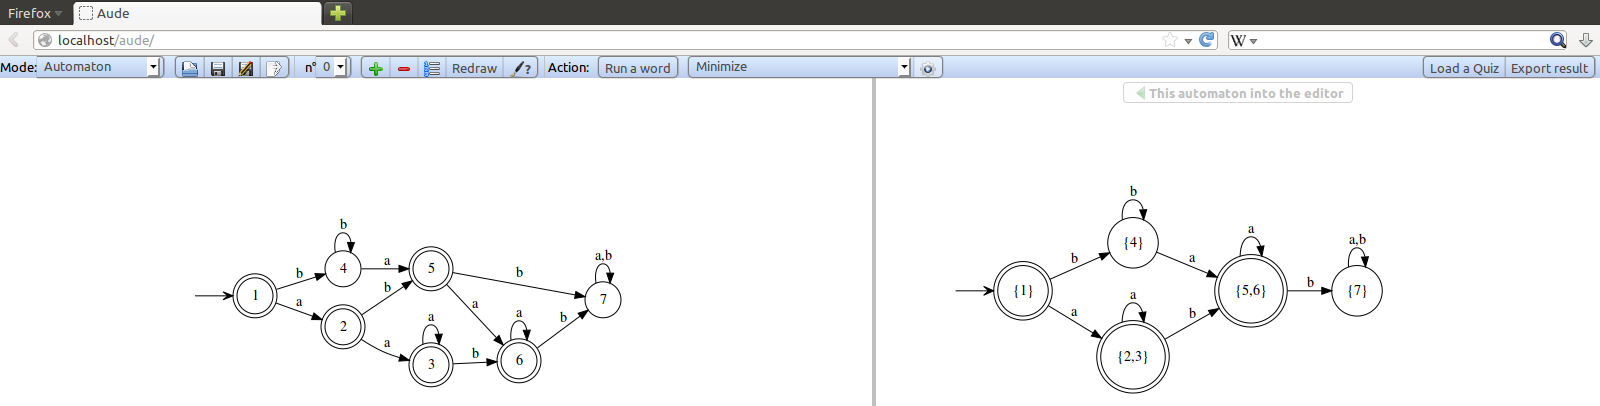
\includegraphics[width=500pt]{{../aude-algo}.png}\caption{Result of an algorithm execution.}\label{aude-algo}\end{figure}


\newpage

\paragraph{}
In addition, students can write their own algorithms using the same dedicated language as the one used for writing embedded algorithms (See figure \ref{aude-prog}).

\begin{figure}[htb]\centering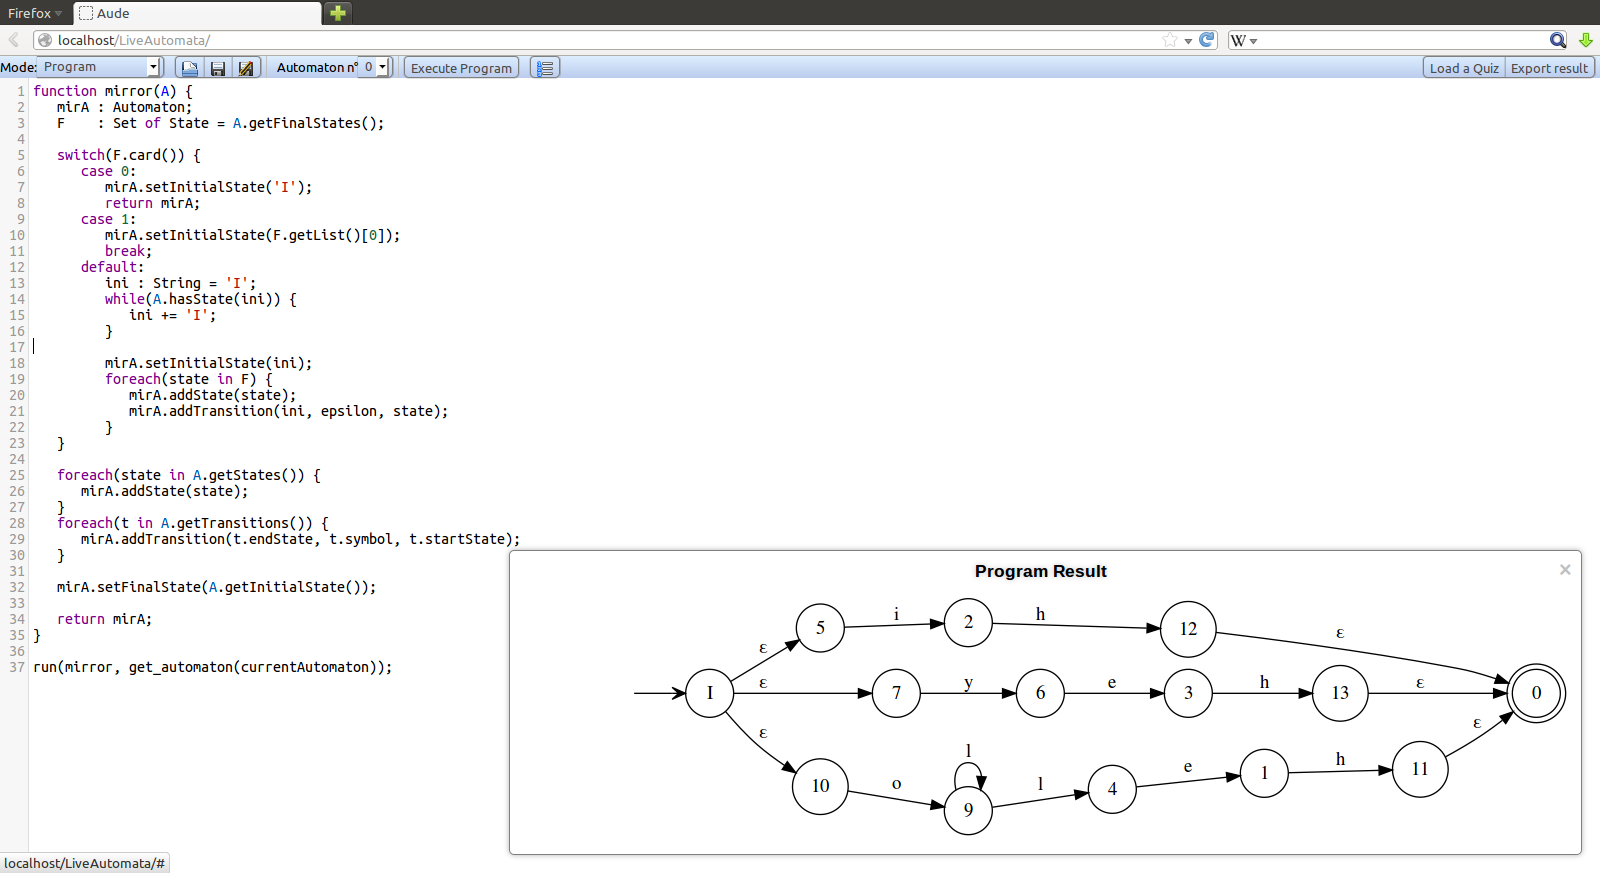
\includegraphics[width=500pt]{{../aude-prog}.png}\caption{Writing algorithms.}\label{aude-prog}\end{figure}


\paragraph{}
Algorithms can take several automata parameters. The user will be asked to choose which automata should be sent to the algorithm when running it.

    \begin{figure}[htb]\centering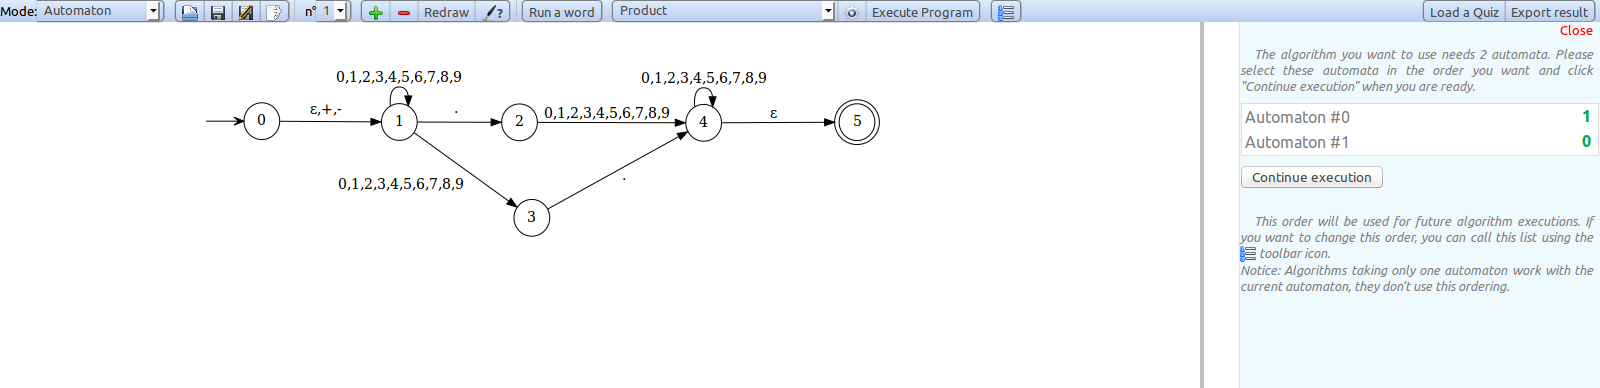
\includegraphics[width=500pt]{{../aude-list-automata}.png}\caption{Choosing which automata should be sent to the algorithm.}\label{aude-list}\end{figure}



\subsection{Running words}

\paragraph{}
Finite state automata are all about word recognition and the execution of a word is probably the most important thing to understand in the automata theory before going any farther. As a result, special care when transmitting the idea of word execution to students must be all the more taken.
The tool features animated word execution and particular attention was taken to make it easy to follow. Students can test words on their drawn and see what path(s) lead to word acceptation or from which state(s) the word was rejected (See figure \ref{word-exec}).

\begin{figure}[htb]\centering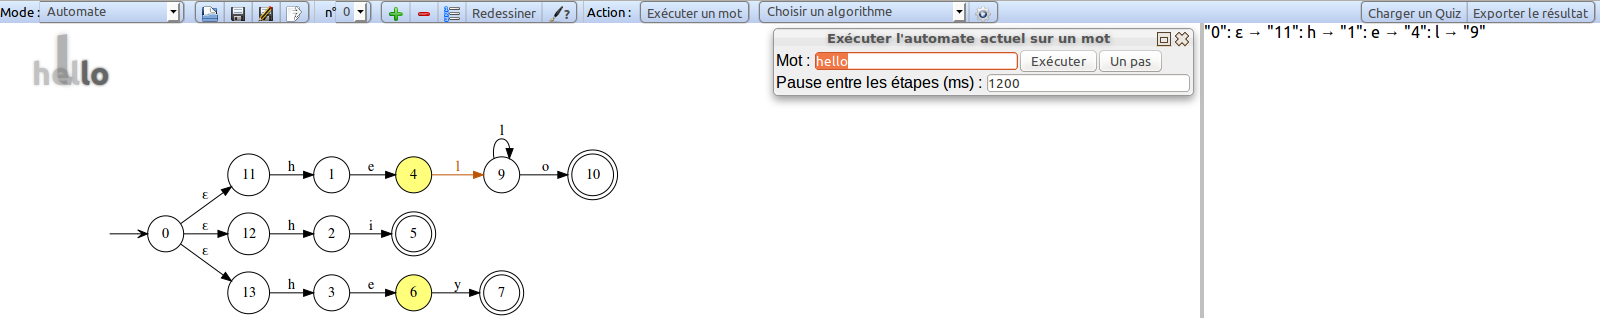
\includegraphics[width=500pt]{{../word-execution}.png}\caption{Word execution.}\label{word-exec}\end{figure}



\subsection{Quizzes}


\paragraph{}
Motivation is important, if not essential, in the process of acquiring knowledge. Interactivity sometimes helps in keeping students motivated and autonomous work can also be sought by a part of the students. \\
We tried to address the issue by implementing a Quiz module in the tool (see figure \ref{aude-quiz}). Teachers (or even students) can write custom quizzes for students so that they can train in autonomy: the tool asks questions, gathers students' responses and tell them what is right and what is wrong.

\paragraph{}
Quizzes can include:

\begin{itemize}
   \item{ mere multiple choice questions, with zero, one or more answers, with any number of possible answers.}
   \item{ questions that ask the user to draw an automaton corresponding to a set of words.}
   \item{ questions that ask the user to draw an automaton corresponding to a language defined by an automaton or a regular expression in the quiz file.}
\end{itemize}

\paragraph{}
The tool supports writing mathematics in the quiz.

\begin{figure}[htb]\centering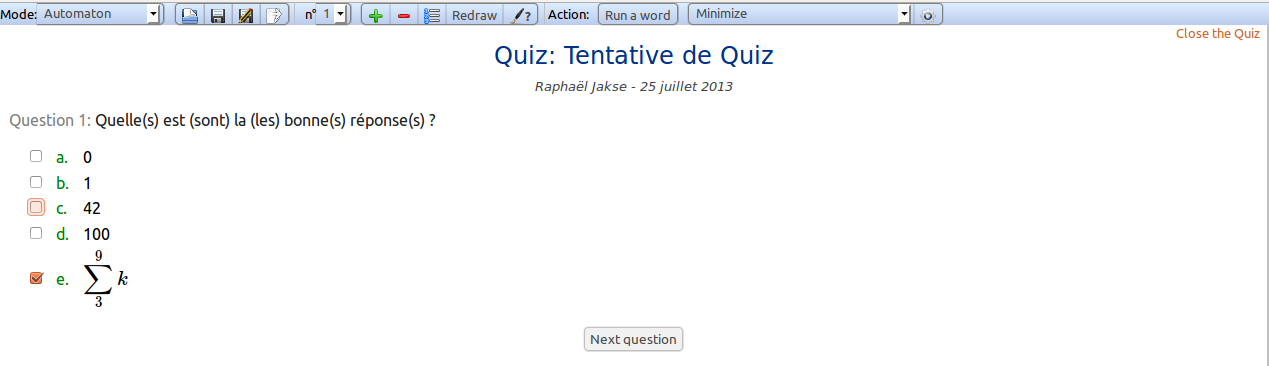
\includegraphics[width=430pt]{{../aude-quiz}.png}\caption{Quiz.}\label{aude-quiz}\end{figure}

\subsection{Automata Theory-compatible Programming Language}
\paragraph{}
The finite state automaton is usually represented by a quintuplet $(Q, \Sigma, \delta, q_0, F)$ where:
\begin{itemize}
   \item{$ Q $ is a \emph{set} of states.}
   \item{$ \Sigma $ is an alphabet. In other words, $ \Sigma $ is a \emph{set} of symbols.}
   \item{$ \delta $ is a transition relation. Put in another way, more precisely, it is a \emph{set} of triplets $(\rm{state}, \rm{symbol}, \rm{state})$.}
   \item{$ q_0 $ is the start state.}
   \item{$ F $ is a \emph{set} of states considered as final, or accepting.}
\end{itemize}

\paragraph{}
The usual definition of the finite state automaton is entirely based and completely depends on sets, and so are automata-related algorithms (see figure~\ref{algo-diff}). As a result, the tool embeds a programming language in which sets are first-class citizens. Instead of writing an entirely new programming language, choice was made to extend Javascript to sets and automata. This implies that students have access to all the features of a widespread generalist programming language as well as features specific to the Automata Theory. See figure~\ref{audejs-ex} to see an implementation of the algorithm~\ref{algo-diff}.

\begin{algorithm}
   \caption{Find differentiable states}
   \label{algo-diff}
   \begin{algorithmic}
      \State \textbf{Input:} $A=(Q, \Sigma, \delta, q_{\rm{init}}, F):$ a deterministic state automaton which all states are accessible.
      \State \textbf{Output:} $D\subseteq Q \times Q$: differentiation relation between states of $ Q $
      \State \textbf{Variables:} $D, D_{\rm{pre}}, X$: sets of state couples
      \State $D \gets \left(F\times (Q \setminus F)\right)$
      \State $D_{\rm{pre}} \gets \{\}$
      \While{$D_{\rm{pre}}\neq D$}
        \State $D_{\rm{pre}}=D$
        \State $X \gets \left\{(p,q) \in Q\: | \: \exists a \in \Sigma, \left(\delta(p,a), \delta(q,a)\right) \in D\right\}$
        \State $D \gets D \cup X$
      \EndWhile
      \State \Return $D$
   \end{algorithmic}
\end{algorithm}

\lstset{language=JavaScript}

\begin{figure}
\label{audejs-ex}
\caption{}
\begin{lstlisting}
function distinguableStates(A) {
   let F     = A.getFinalStates(),
       Q     = A.getStates(),
       Sigma = A.getAlphabet(),
       delta = A.getTransitionFunction(true);

   D     : Set of List = F cross (Q minus F);
   D_pre : Set of List = emptySet;
   X     : Set of List;
   while(D != D_pre) {
      D_pre = D.copy();

      X = emptySet;
      foreach(p in Q) {
         foreach(q in Q) {
            foreach(a in Sigma) {
               if([delta(p, a), delta(q, a)] belongsTo D) {
                  X.add([p, q]);
               }
            }
         }
      }

      D Union= X;
   }
   return D;
}
\end{lstlisting}
\end{figure}
\paragraph{}
Extending a programming language, in our case, means:

\begin{itemize}
   \item{Extending the ``standard library'': adding a class to manipulate sets and a class to manipulate automata.}
   \item{Modifying the grammar of the language: adding features like set manipulations and iteration.}
\end{itemize}

\paragraph{}
Concretely, the tool embeds a function which maps a code written in our programming language to a pure Javascript code. This Javascript code can then be executed in any Javascript-compatible Web browser.
The mapping is done with the following constraints:
\begin{itemize}
   \item{ $ n $\textsuperscript{th} line  of the generated code must correspond to the $ n $\textsuperscript{th}  line of the input code, for accuracy in error reporting}
   \item{ The generated code must be identical to the input code if the input code is pure Javascript.}
\end{itemize}

\paragraph{}
Since sets look like Javascript blocks of code, transformations must not be done inside strings, and some transformations can be nested, regular expressions are not sufficient to handle the translation.

\DefineShortVerb{\#}
\SaveVerb{v1}#foreach(i in object) { ... }#
\SaveVerb{v3}#varname : Type#
\SaveVerb{v4}#var varname = new Type#
\UndefineShortVerb{\#}

\lstset{numbers=none, frame=none}

\newsavebox\foreachinput
\begin{lrbox}{\foreachinput}
\begin{minipage}{0.5\textwidth}
 \begin{lstlisting}
foreach(e in mySet) {
  if(e == {1,2,3}) {
   break; // we found our triplet
  }
  else if(e instanceof Set) { // if e is a Set
    try{(e).forEach(function(f ) {
      if( contains(e, epsilon)) {
        throw 0; //we found epsilon
      }
    }
  )}catch(e){if(e instanceof Error){throw e}else if(!(e === StopIteration)){throw e;}}}

  if(  Audescript.eq(e, new Set())) {
     throw -1; // we found the empty set. Stopping the execution.
  }
}

// ...
)}catch(e){if(e instanceof Error){throw e}else if(!(e === StopIteration)){return e;}}
 \end{lstlisting}
\end{minipage}
\end{lrbox}


\newsavebox\foreachgenerated
\begin{lrbox}{\foreachgenerated}
\begin{minipage}{0.5\textwidth}
 \begin{lstlisting}
try{(object).forEach(function (i ) {

}
)}catch (e) {if (e instanceof audescript.ThrowValue) {throw e.v;}else if (e instanceof audescript.ReturnValue) {return e.v;}}
 \end{lstlisting}
\end{minipage}
\end{lrbox}

\noindent\begin{tabularx}{\linewidth}{|*{2}{X|}}
\hline
{\bfseries  Input code                              } & {\bfseries  Generated code             }\tabularnewline
\hline
 \UseVerb{v1}  & \usebox\foreachgenerated \tabularnewline
\hline
 \UseVerb{v3}                &  \UseVerb{v4}       \tabularnewline
\hline
\end{tabularx}

\paragraph{}
These transformations must not be done inside string literals, {\itshape object} in \lstinline!foreach! can contain parenthesis, the variable declaration can hold a initialization value, set literals look very similar to blocks of codes, \lstinline!foreach! can be nested so a need to match curly brackets appears, \lstinline!break! and \lstinline!return! statement must be transformed inside \lstinline!foreach! loop, etc. Manipulated languages are not {\itshape regular}\footnote{a language is regular iff it can be described with a regular expression. Rules like “there is the same number of opening and closing parenthesis” make a language not regular.} and transformations are not that trivial eventually. As a consequence, another method needs to be used, the code must be parsed more subtly.

\paragraph{}
A project like \href{http://zaach.github.io/jison/}{Jison}, which is a parser like \href{http://www.gnu.org/software/bison/}{Bison} might have been used\footnote{See \href{http://cjihrig.com/blog/creating-a-javascript-parser/}{http://cjihrig.com/blog/creating-a-javascript-parser/} for an implementation of a Javascript parser with Jison}. However, handwriting the parser was chosen in order to keep whitespace characters intact, to have full control over optional semicolons (if a semicolon was not written by the programmer, the semicolon should not appear in the generated code) and to handle ambiguities between regular expression tokens (which begin with \lstinline!/!) and division operators (\lstinline!/!, \lstinline!/=!) easily. Handwriting the parser also seemed to be a more efficient and straightforward solution here because transformations can be made without generating any abstract syntax tree. Moreover, this lets write a quite flexible parser, validation being delegated to the actual Javascript engine, which already has a good error reporting system.

\section{Comparison with other tools}

\paragraph{}
Like most tools of the domain, the tool gives the ability to the user to draw automata. However, unlike its friends, the user has more freedom in {\em choosing the shape of the transitions}, though Visual Automata Simulator is great for this, and thanks to the tight integration of Graphviz, automata can be {\em (re)drawn automatically} and have a {\em familiar look}.
   
   
\paragraph{}
Like most others tools, the program comes with basic common algorithms related to automata. However, it comes with {\em far more algorithms} than its friends and {\em lets the user write its own algorithms easily}, providing a language close to Javascript with sets as first-class citizens, which makes it suitable for manipulation of automata.

   
\paragraph{}
The program is designed with the user in mind: everything is thought to be the more pleasant and natural possible, appearance not being set aside. An example of this is the graphical execution of a word: current states are seen in yellow, transitions being taken right now are brown and current final states are green. If a word runs out of the automaton, its states are drawn in red. The execution can be made {\em step by step} or not and animations were designed to ease the visualization of the execution.

   
\paragraph{}
What also make the program stand out is the Quiz Feature: it gives the ability to teachers and students to {\em write quiz for students} and these quizzes are run by the tool, using its automata manipulation capabilities. Questions of the quiz can be mere multiple choices questions as well as asking the user to write automata or regular expressions.
   
   
\paragraph{}
Another thing that can be said is that unlike others tools, this one is written with web technologies, which makes the program usable without any installation and will make the port on tablets easy. Thanks to web technologies, the program should work on any desktop operating system, provided a recent browser is installed, and the support for mobile operating systems should follow quickly.

   
\newpage
   
\paragraph{}
The following table\footnote{Icons in the table come from the Oxygen theme: \href{http://www.oxygen-icons.org/}{http://www.oxygen-icons.org/}} compares Aude with some other tools of the domain.

      \noindent\begin{tabularx}{\linewidth}{|*{6}{X|}}
\hline
{\bfseries  Feature                    } & {\bfseries  Aude         } & {\bfseries  jFAST} & {\bfseries jFLAP  } & {\bfseries  Visual Automata Simulator (VAS) } & {\bfseries Finite Automata Tool (FAT)}\tabularnewline
\hline
 Finite-state automata        &  
\includegraphics[height=14pt]{{../dialog-ok-apply}.png}            &  
\includegraphics[height=14pt]{{../dialog-ok-apply}.png}    &  
\includegraphics[height=14pt]{{../dialog-ok-apply}.png}     &  
\includegraphics[height=14pt]{{../dialog-ok-apply}.png}                        &  
\includegraphics[height=14pt]{{../dialog-ok-apply}.png}\tabularnewline
\hline
 Turing Machine               &  
\includegraphics[height=14pt]{{../edit-delete}.png}             &  
\includegraphics[height=14pt]{{../edit-delete}.png}     &  
\includegraphics[height=14pt]{{../dialog-ok-apply}.png}     &  
\includegraphics[height=14pt]{{../dialog-ok-apply}.png}                        &  
\includegraphics[height=14pt]{{../edit-delete}.png}\tabularnewline
\hline
 Mealy Machine                &  
\includegraphics[height=14pt]{{../edit-delete}.png}             &  
\includegraphics[height=14pt]{{../edit-delete}.png}     &  
\includegraphics[height=14pt]{{../dialog-ok-apply}.png}     &  
\includegraphics[height=14pt]{{../edit-delete}.png}                         &  
\includegraphics[height=14pt]{{../edit-delete}.png}\tabularnewline
\hline
 More Machine                 &  
\includegraphics[height=14pt]{{../edit-delete}.png}             &  
\includegraphics[height=14pt]{{../edit-delete}.png}     &  
\includegraphics[height=14pt]{{../dialog-ok-apply}.png}     &  
\includegraphics[height=14pt]{{../edit-delete}.png}                         &  
\includegraphics[height=14pt]{{../edit-delete}.png}\tabularnewline
\hline
 Pushdown automaton           &  
\includegraphics[height=14pt]{{../edit-delete}.png}             &  
\includegraphics[height=14pt]{{../edit-delete}.png}     &  
\includegraphics[height=14pt]{{../dialog-ok-apply}.png}     &  
\includegraphics[height=14pt]{{../edit-delete}.png}                         &  
\includegraphics[height=14pt]{{../edit-delete}.png}\tabularnewline
\hline
 Grammar Manipulation         &  
\includegraphics[height=14pt]{{../edit-delete}.png}             &  
\includegraphics[height=14pt]{{../edit-delete}.png}     &  
\includegraphics[height=14pt]{{../dialog-ok-apply}.png}     &  
\includegraphics[height=14pt]{{../edit-delete}.png}                         &  
\includegraphics[height=14pt]{{../edit-delete}.png}  \tabularnewline
\hline
 Draw automata                &  
\includegraphics[height=14pt]{{../dialog-ok-apply}.png}            &  
\includegraphics[height=14pt]{{../dialog-ok-apply}.png}    &  
\includegraphics[height=14pt]{{../dialog-ok-apply}.png}     &  
\includegraphics[height=14pt]{{../dialog-ok-apply}.png}                        &  
\includegraphics[height=14pt]{{../edit-delete}.png}\tabularnewline
\hline
 Regular expression to FSA    &  
\includegraphics[height=14pt]{{../dialog-ok-apply}.png}            &  
\includegraphics[height=14pt]{{../edit-delete}.png}     &  
\includegraphics[height=14pt]{{../dialog-ok-apply}.png}     &  
\includegraphics[height=14pt]{{../edit-delete}.png}                         &  
\includegraphics[height=14pt]{{../edit-delete}.png}\tabularnewline
\hline
 Run a word                   &  
\includegraphics[height=14pt]{{../dialog-ok-apply}.png}            &  Complete DFA only  &  
\includegraphics[height=14pt]{{../dialog-ok-apply}.png}  &  no epsilon transition  &  
\includegraphics[height=14pt]{{../edit-delete}.png}\tabularnewline
\hline
 Apply basic algorithms       &  
\includegraphics[height=14pt]{{../dialog-ok-apply}.png}            &  
\includegraphics[height=14pt]{{../edit-delete}.png}     &  Determinization, minimization, completion  &   Determinization  &  Union, Intersection, Complementation, Minimization, Determinization\tabularnewline
\hline
 Combine two automata         &  \includegraphics[height=14pt]{{../edit-delete}.png}             &  \includegraphics[height=14pt]{{../edit-delete}.png}     &  \includegraphics[height=14pt]{{../dialog-ok-apply}.png}     &  \includegraphics[height=14pt]{{../edit-delete}.png}                        &  \includegraphics[height=14pt]{{../edit-delete}.png}\tabularnewline
\hline
 Quiz                         &  \includegraphics[height=14pt]{{../dialog-ok-apply}.png}            &  \includegraphics[height=14pt]{{../edit-delete}.png}     &  \includegraphics[height=14pt]{{../edit-delete}.png}      &  \includegraphics[height=14pt]{{../edit-delete}.png}                        &  \includegraphics[height=14pt]{{../edit-delete}.png}\tabularnewline
\hline
 Games                        &  \includegraphics[height=14pt]{{../edit-delete}.png}             &  \includegraphics[height=14pt]{{../edit-delete}.png}     &  Pumping Lemma  &  \includegraphics[height=14pt]{{../edit-delete}.png}                 &  \includegraphics[height=14pt]{{../edit-delete}.png}\tabularnewline
\hline
 User's algorithms            &  \includegraphics[height=14pt]{{../dialog-ok-apply}.png}            &  \includegraphics[height=14pt]{{../edit-delete}.png}     &  \includegraphics[height=14pt]{{../edit-delete}.png}      &  \includegraphics[height=14pt]{{../edit-delete}.png}                        &  \includegraphics[height=14pt]{{../edit-delete}.png}\tabularnewline
\hline
 Consult built-in algorithms  &  \includegraphics[height=14pt]{{../dialog-ok-apply}.png}            &  \includegraphics[height=14pt]{{../edit-delete}.png}     &  \includegraphics[height=14pt]{{../edit-delete}.png}      &  \includegraphics[height=14pt]{{../edit-delete}.png}                        &  \includegraphics[height=14pt]{{../edit-delete}.png}\tabularnewline
\hline
 Automatic automaton drawing  &  \includegraphics[height=14pt]{{../dialog-ok-apply}.png}            &  \includegraphics[height=14pt]{{../edit-delete}.png}     &  \includegraphics[height=14pt]{{../edit-delete}.png}      &  \includegraphics[height=14pt]{{../edit-delete}.png}                        &  \includegraphics[height=14pt]{{../edit-delete}.png}\tabularnewline
\hline
 Automaton code input         &  \includegraphics[height=14pt]{{../dialog-ok-apply}.png}            &  \includegraphics[height=14pt]{{../edit-delete}.png}     &  \includegraphics[height=14pt]{{../edit-delete}.png}      &  \includegraphics[height=14pt]{{../edit-delete}.png}                        &  \includegraphics[height=14pt]{{../dialog-ok-apply}.png}\tabularnewline
\hline
 Run online                   &  \includegraphics[height=14pt]{{../dialog-ok-apply}.png}            &  Java RE  &  Java RE  &  Java RE  &  Java RE\tabularnewline
\hline
 Requires                     &  A Web browser  &  Java   &  Java    &  Java                      &  Java\tabularnewline
\hline
\end{tabularx}


\section{Future work}

\section{Conclusion}


\end{sloppypar}
\end{document}
